Nicht jede Software wird als Standalone Anwendung ausgeführt, es kann auch passieren, dass man 
erst ein Kern umsetzt, die dann in jeweiligen Anwendungen entsprechend angepasst werden 
oder es handelt sich nur um eine Komponente für die andere Anwednung.
Eine Analogie aus OOP wäre eine Abstrakte Klasse.

Grundsätzlich kann man die Abbildung \ref{fig:sp2d} folgendeweise vereinfachen:
\begin{figure}[H]
    \centering
    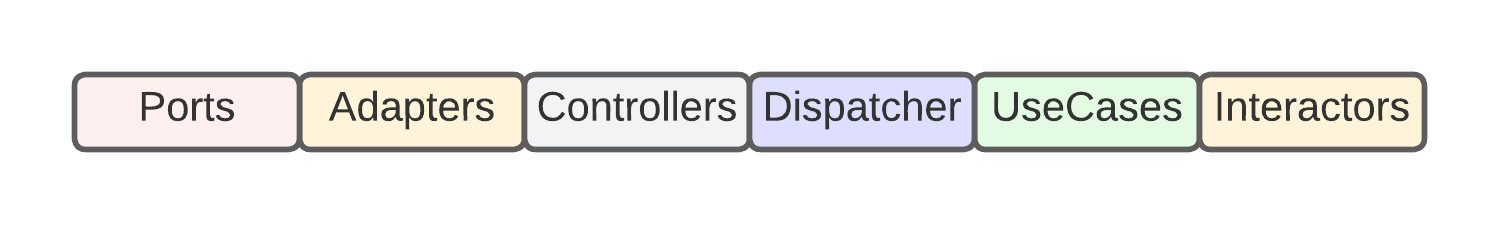
\includegraphics[width=1\textwidth]{./images/SimpliedArchitecture.png}
    \caption{Vereinfachte Darstellung}
    \label{fig:SimpliedArchitecture}
    \source{Eigene Quelle}
\end{figure}

Und bei einer Standalone Anwendung gibt es eine Main-Methode, die diese Struktrur erstellt.
\begin{figure}[H]
    \centering
    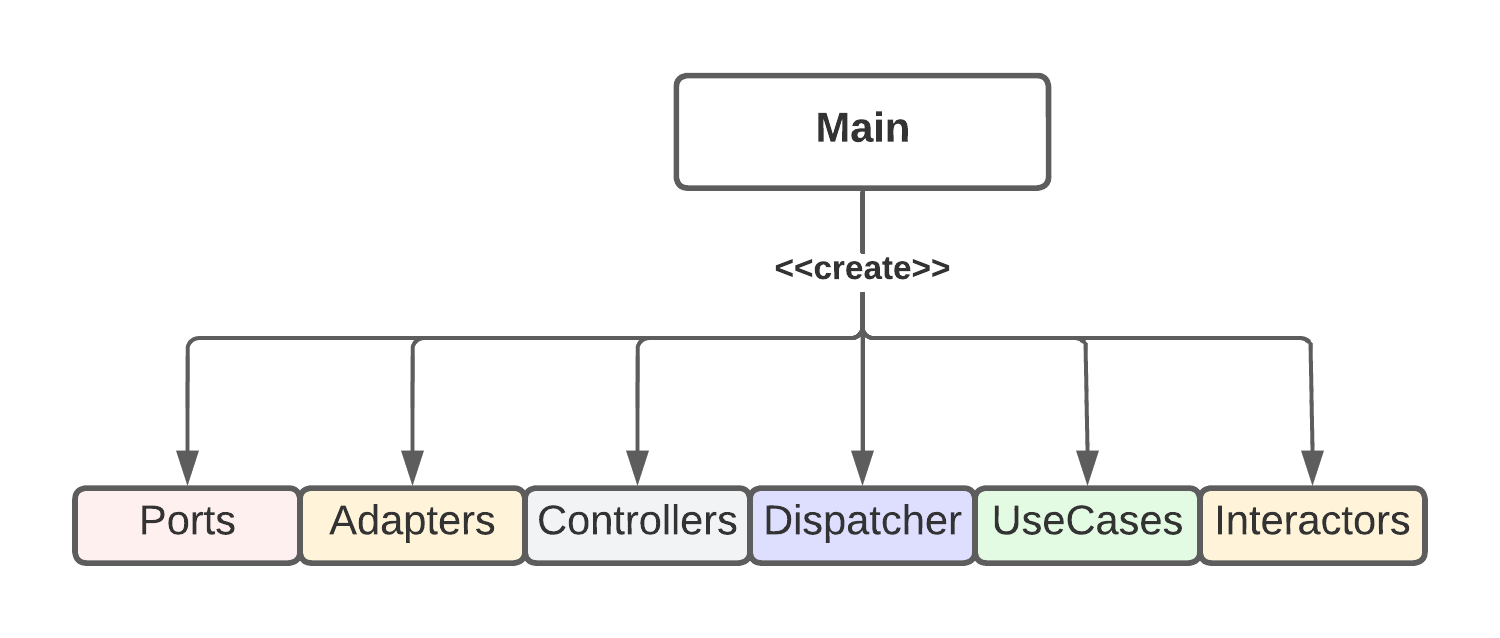
\includegraphics[width=1\textwidth]{./images/Architecture as Standalone.png}
    \caption{Vereinfachte Darstellung einer Standalone Anwendung}
    \label{fig:SimpliedArchitectureAsStandalone}
    \source{Eigene Quelle}
\end{figure}

Der Datenfluss lässt sich so darstellen:
\begin{figure}[H]
    \centering
    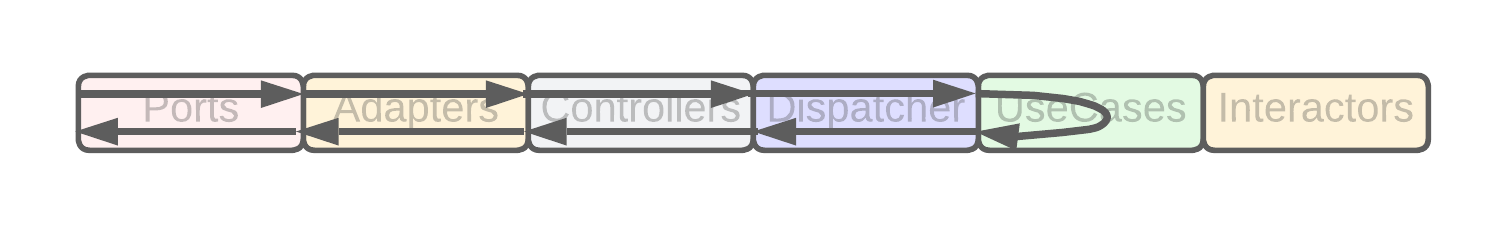
\includegraphics[width=1\textwidth]{./images/Dataflow.png}
    \caption{Vereinfachte Darstellung einer Standalone Anwendung}
    \label{fig:SimpliedArchitectureDataflow}
    \source{Eigene Quelle}
\end{figure}

\newpage
Wenn man es als Komponente in einer anderen Anwendung benutzen möchte, braucht die Struktur eine Facade, damit man 
auf "wichtige Teile" der Komponente zugreifen kann und der Rest verborgen bleibt. 
Die Facade baut die gesamte Struktur der Komponente auf.

So sieht eine fertige Komponente aus, die man in die anderen Anwendungen integrieren kann:

\begin{figure}[H]
    \centering
    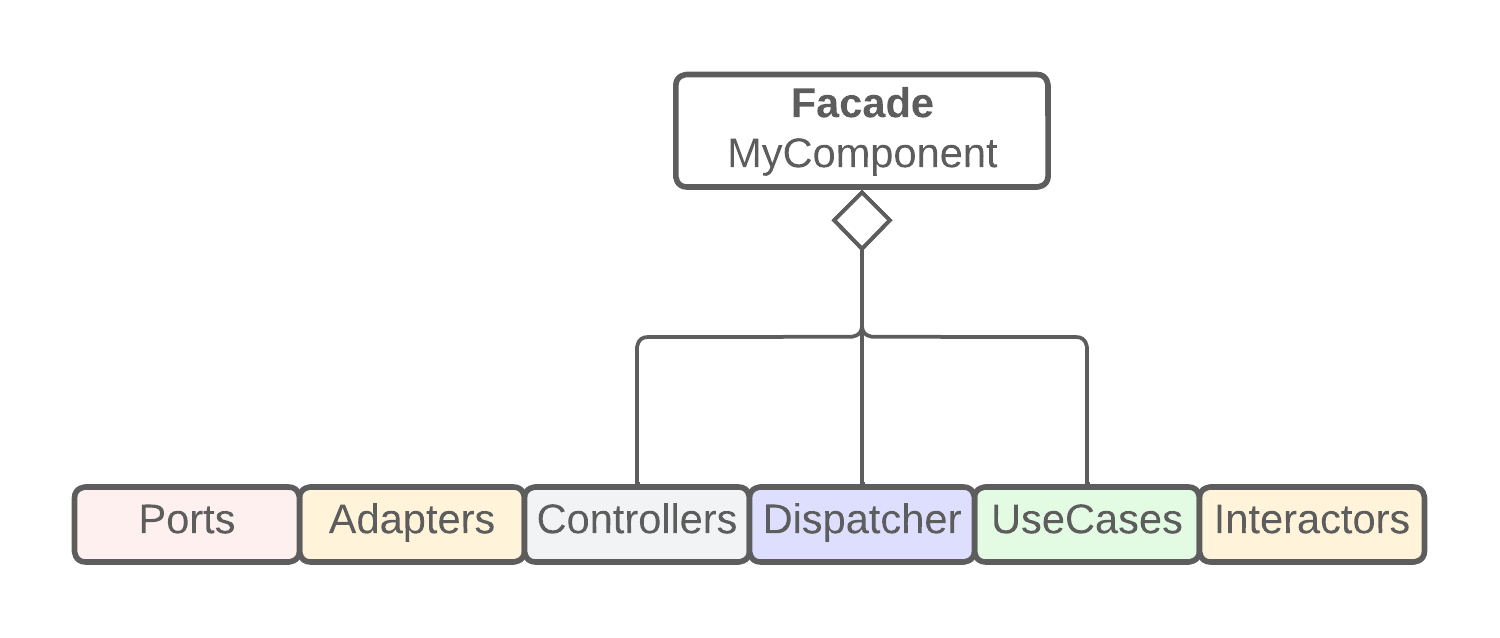
\includegraphics[width=1\textwidth]{./images/Architecture as Facade.png}
    \caption{Vereinfacte Darstellung der Architektur als Komponente}
    \label{fig:SimpliedArchitectureAsKomponent}
    \source{Eigene Quelle}
\end{figure}

Auf der Darstellung \ref{fig:SimpliedArchitectureAsKomponent} sieht man, dass die Anwendung nur den Zugriff auf drei Teile der Komponente hat.
Das sind:
\begin{itemize}
    \item \textbf{Controllers} - um die Zustände des jeweiligen Controllers abfragen und ändern.
    \item \textbf{Dispatcher} - um alle Ereignise in der Komponente abzufangen.
    \item \textbf{UseCases} - um das Verhalten auf gewisse Ereignise ändern zu können.
\end{itemize}

Die Komponente kann bestimmte Ereignise selber abarbeiten und die Anwendung davon gar nicht informieren oder
das Ereignis weiterleiten, dass es von der Anwednung selbst abarbeitet wird.
Die Komponente wird von der eigentlichen Anwendung unabhängig entwickelt, somit wird es passieren, dass
der Datentyp des Ereignisses von der Komponente nicht mit dem Datentyp der Anwendung übereinstimmt und deswegen muss noch durch den entsprechenden Adapter angepasst werden.
Das bedeutet, dass die Komponente wird nur von dem \textbf{Port} der jeweiligen Anwendung benutzt wird.

\newpage
Die Vereinfacte Darstellung der Anwendung mit der Komponente:
\begin{figure}[H]
    \centering
    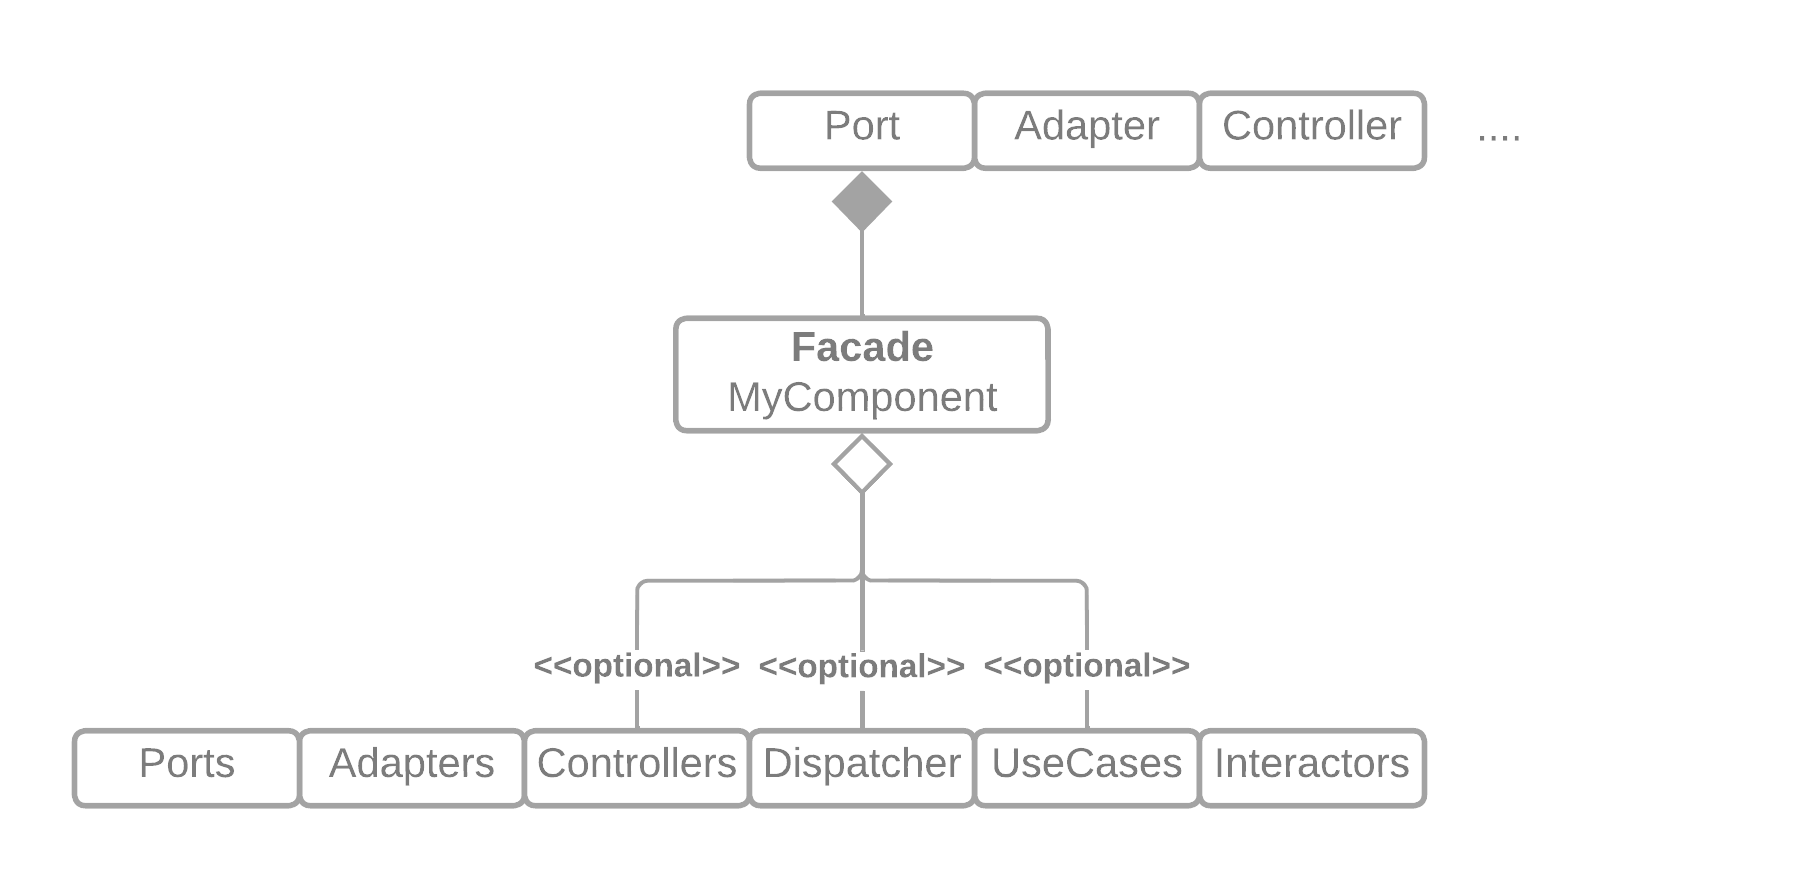
\includegraphics[width=1\textwidth]{./images/Architecture as Component.png}
    \caption{Vereinfacte Darstellung einer Standalone Anwendung mit der Komponente}
    \label{fig:SimpliedArchitectureAsStandaloneWithComponent}
    \source{Eigene Quelle}
\end{figure}

Der Datenfluss in der Anwendung würde wie folgt aussehen:
\begin{figure}[H]
    \centering
    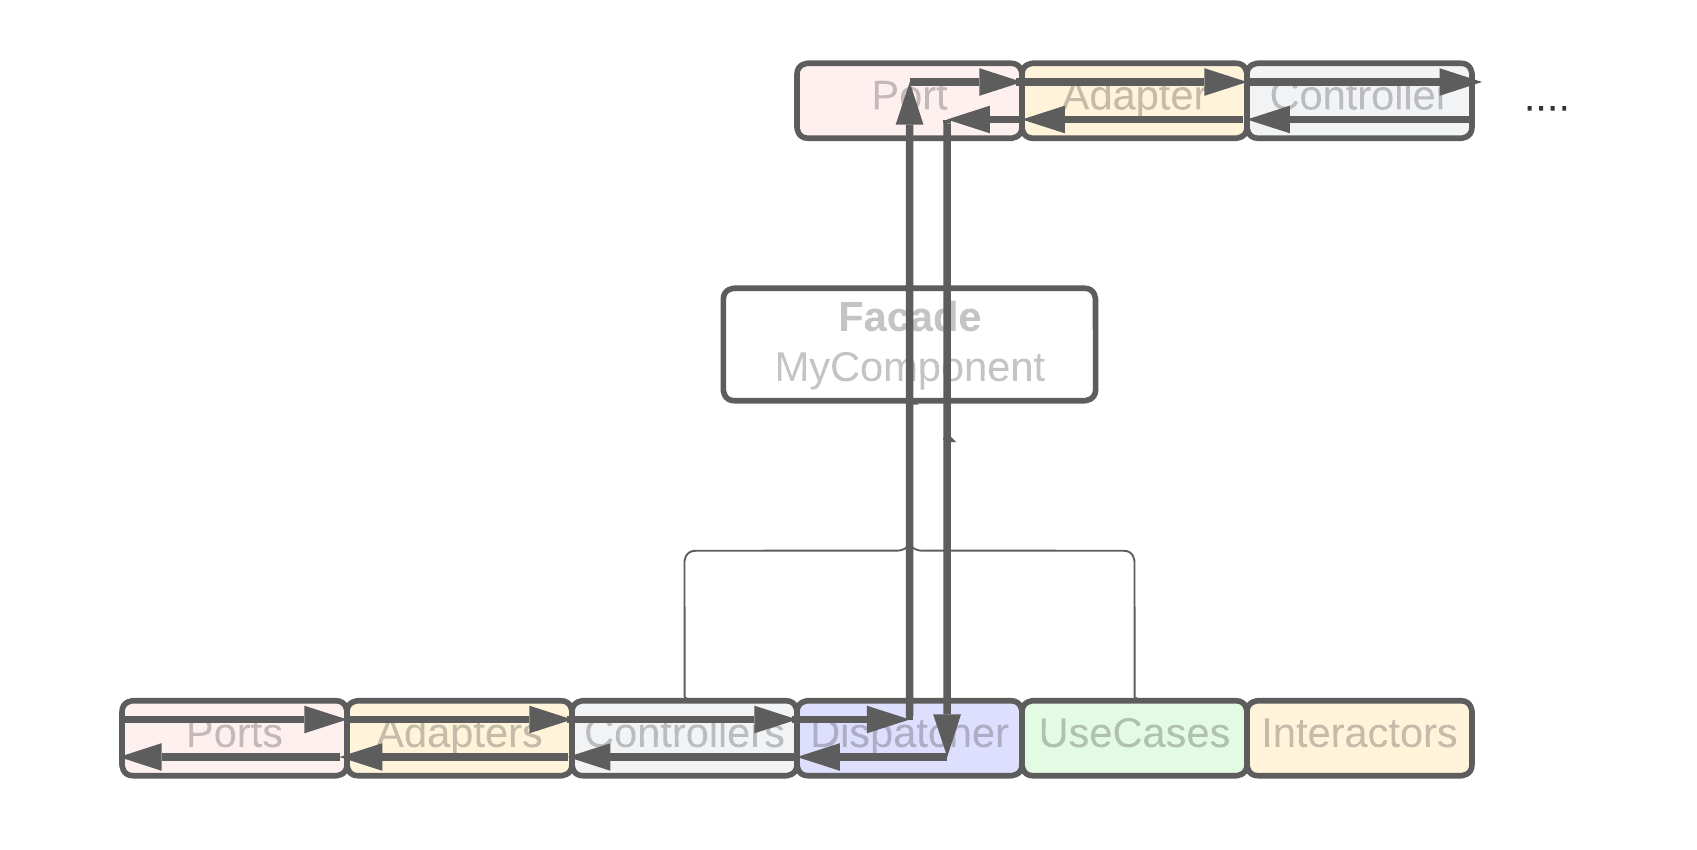
\includegraphics[width=1\textwidth]{./images/Dataflow as Component with inform.png}
    \caption{Vereinfacte Darstellung des Datenflusses in einer Anwendung mit Komponente}
    \label{fig:SimpliedDataflowWithComponent}
    \source{Eigene Quelle}
\end{figure}